%% Submissions for peer-review must enable line-numbering
%% using the lineno option in the \documentclass command.
%%
%% Preprints and camera-ready submissions do not need
%% line numbers, and should have this option removed.
%%
%% Please note that the line numbering option requires
%% version 1.1 or newer of the wlpeerj.cls file, and
%% the corresponding author info requires v1.2

\documentclass[fleqn,10pt]{wlpeerj} % for preprint submissions

% ZNK -- Adding headers for pandoc

\setlength{\emergencystretch}{3em}
\providecommand{\tightlist}{
\setlength{\itemsep}{0pt}\setlength{\parskip}{0pt}}
\usepackage{lipsum}
\usepackage[unicode=true]{hyperref}
\usepackage{longtable}



\usepackage{booktabs}
\usepackage{array}
\usepackage{multirow}
\usepackage{wrapfig}
\usepackage{float}
\usepackage{colortbl}
\usepackage{pdflscape}
\usepackage{tabu}
\usepackage{threeparttable}
\usepackage{threeparttablex}
\usepackage[normalem]{ulem}
\usepackage{makecell}
\usepackage{xcolor}

\title{Visualisation of Brain Statistics with R-package \texttt{ggseg}}

\author[1]{Athanasia M. Mowinckel}

\corrauthor[1]{Athanasia M. Mowinckel}{\href{mailto:a.m.mowinckel@psykologi.uio.no}{\nolinkurl{a.m.mowinckel@psykologi.uio.no}}}
\author[1]{Didac Vidal Piñeiro}


\affil[1]{Center for Lifespan Changes in Brain and Cognition, Univeristy of Oslo, PO. box 1094 Blindern, 0317 Oslo, Norway}


%
% \author[1]{First Author}
% \author[2]{Second Author}
% \affil[1]{Address of first author}
% \affil[2]{Address of second author}
% \corrauthor[1]{First Author}{f.author@email.com}

% 
\usepackage{natbib}
\bibliographystyle{plainnat}

\begin{abstract}
The abstract of the article. It can also be on \emph{multiple} lines.
% Dummy abstract text. Dummy abstract text. Dummy abstract text. Dummy abstract text. Dummy abstract text. Dummy abstract text. Dummy abstract text. Dummy abstract text. Dummy abstract text. Dummy abstract text. Dummy abstract text.
\end{abstract}

\usepackage{color}
\usepackage{fancyvrb}
\newcommand{\VerbBar}{|}
\newcommand{\VERB}{\Verb[commandchars=\\\{\}]}
\DefineVerbatimEnvironment{Highlighting}{Verbatim}{commandchars=\\\{\}}
% Add ',fontsize=\small' for more characters per line
\usepackage{framed}
\definecolor{shadecolor}{RGB}{248,248,248}
\newenvironment{Shaded}{\begin{snugshade}}{\end{snugshade}}
\newcommand{\AlertTok}[1]{\textcolor[rgb]{0.94,0.16,0.16}{#1}}
\newcommand{\AnnotationTok}[1]{\textcolor[rgb]{0.56,0.35,0.01}{\textbf{\textit{#1}}}}
\newcommand{\AttributeTok}[1]{\textcolor[rgb]{0.77,0.63,0.00}{#1}}
\newcommand{\BaseNTok}[1]{\textcolor[rgb]{0.00,0.00,0.81}{#1}}
\newcommand{\BuiltInTok}[1]{#1}
\newcommand{\CharTok}[1]{\textcolor[rgb]{0.31,0.60,0.02}{#1}}
\newcommand{\CommentTok}[1]{\textcolor[rgb]{0.56,0.35,0.01}{\textit{#1}}}
\newcommand{\CommentVarTok}[1]{\textcolor[rgb]{0.56,0.35,0.01}{\textbf{\textit{#1}}}}
\newcommand{\ConstantTok}[1]{\textcolor[rgb]{0.00,0.00,0.00}{#1}}
\newcommand{\ControlFlowTok}[1]{\textcolor[rgb]{0.13,0.29,0.53}{\textbf{#1}}}
\newcommand{\DataTypeTok}[1]{\textcolor[rgb]{0.13,0.29,0.53}{#1}}
\newcommand{\DecValTok}[1]{\textcolor[rgb]{0.00,0.00,0.81}{#1}}
\newcommand{\DocumentationTok}[1]{\textcolor[rgb]{0.56,0.35,0.01}{\textbf{\textit{#1}}}}
\newcommand{\ErrorTok}[1]{\textcolor[rgb]{0.64,0.00,0.00}{\textbf{#1}}}
\newcommand{\ExtensionTok}[1]{#1}
\newcommand{\FloatTok}[1]{\textcolor[rgb]{0.00,0.00,0.81}{#1}}
\newcommand{\FunctionTok}[1]{\textcolor[rgb]{0.00,0.00,0.00}{#1}}
\newcommand{\ImportTok}[1]{#1}
\newcommand{\InformationTok}[1]{\textcolor[rgb]{0.56,0.35,0.01}{\textbf{\textit{#1}}}}
\newcommand{\KeywordTok}[1]{\textcolor[rgb]{0.13,0.29,0.53}{\textbf{#1}}}
\newcommand{\NormalTok}[1]{#1}
\newcommand{\OperatorTok}[1]{\textcolor[rgb]{0.81,0.36,0.00}{\textbf{#1}}}
\newcommand{\OtherTok}[1]{\textcolor[rgb]{0.56,0.35,0.01}{#1}}
\newcommand{\PreprocessorTok}[1]{\textcolor[rgb]{0.56,0.35,0.01}{\textit{#1}}}
\newcommand{\RegionMarkerTok}[1]{#1}
\newcommand{\SpecialCharTok}[1]{\textcolor[rgb]{0.00,0.00,0.00}{#1}}
\newcommand{\SpecialStringTok}[1]{\textcolor[rgb]{0.31,0.60,0.02}{#1}}
\newcommand{\StringTok}[1]{\textcolor[rgb]{0.31,0.60,0.02}{#1}}
\newcommand{\VariableTok}[1]{\textcolor[rgb]{0.00,0.00,0.00}{#1}}
\newcommand{\VerbatimStringTok}[1]{\textcolor[rgb]{0.31,0.60,0.02}{#1}}
\newcommand{\WarningTok}[1]{\textcolor[rgb]{0.56,0.35,0.01}{\textbf{\textit{#1}}}}

\begin{document}

\flushbottom
\maketitle
\thispagestyle{empty}

\hypertarget{introduction}{%
\section{Introduction}\label{introduction}}

Visualization is increasingly important for accurate guidance and interpretation of neuroimaging results, as current research is able to generate a high amount of data and outcomes.
For Magnetic Resonance Imaging (MRI), neuroimaging software provides whole-brain information by using many small units of space (\textgreater{}100.000).
Nonetheless, this data is often grouped and summarized into a limited number of regions using predefined brain parcellation atlases.
Brain parcellations segment the brain into a finite set of meaningful neurobiological components, which reflect one or more brain features either based on local/structural or connectivity properties (\citet{eickhoff_2018}).
The use of brain atlases is widespread as these facilitate interpretation and minimize the amount of data, hence reducing problems with multiple comparisons and facilitating replicability and data sharing in otherwise computationally expensive analyses.
Complex analyses and post-processing is often performed in specialized software environments such as R (\citet{R}).

MRI data provides good spatial resolution and thus an optimal representation has to respect spatial relationships across regions.
Results from brain atlas analyses are most meaningfully visualized when projected onto a representation of the brain, rather than on other types of graphs (e.g.~bar charts).
The projection of data into brain representations provides clear points of reference - especially when the reader is unfamiliar with the atlas - eases readability, guides interpretation, and informs on the spatial patterns of the data.
Adopting the grammar of graphics implemented in ggplot2 (\citet{ggplot}), one can plot neuroimaging data directly in R with several tools such as ggBrain (\citet{ggBrain}) and ggneuro (\citet{ggneuro}; see neuroconductor \citeyearpar{neuroconductor} for curated neuroimaging packages for R).
Yet these tools display whole-brain image files and are not suited for representing brain atlas data.

In this tutorial, we introduce the ggseg-package for visualizing brain atlas data in R.
The ggseg -- and the complimentary ggsegExtra -- package include pre-compiled data sets for different brain atlases that allow for 2D and 3D visualization.
Two-dimensional functionality is based on polygons and ggplot-based grammar of graphics (\citet{ggplot}), while the 3D functionality is based on tri-surface mesh plots and plotly (\citet{plotly}).

The ggseg-package presents both compiled data sets, tailored scripts to allow brain data integration and plotting and, other minor features such as custom color palettes.
The data featured are derived from two well-known parcellations: the Desikan-Killany cortical atlas (DKT; \citet{dkt}), which covers the cortical surface of the brain, and the Automatic Segmentation of Subcortical Structures (aseg; \citet{aseg}), which covers the subcortical structures.
Both atlases are implemented in several neuroimaging softwares, such as FreeSurfer (\citet{fischl_99}, \citet{dale_99}, \citet{Fischl2000}), and are commonly used in relation to developmental changes, disease biomarkers, genomic data, and cognition (\citet{amlien_elaboration_2019}, \citet{WALHOVD20051261}, \citet{Pizzagalli}).
The ggsegExtra-package currently includes \textgreater{}13 additional precompiled atlases and it is continuously expanding.
See Table \ref{tab:atlasTab} for a summary of the available atlases.

We encourage users to contribute to the ggsegExtra brain atlas repository.
In SI text and \href{https://github.com/LCBC-UiO/ggseg/wiki}{github wiki}, we offer a pipeline to create and supply atlases for 2D plotting.
See SI text and SI scripts for instruction to include atlases for 3D plotting.

\begin{table}[t]

\caption{\label{tab:atlasTab}Table of currently available atlases in either ggseg or ggsegExtra R-package. Most atlases have both polygon and mesh atlases, but the mesh atlases are somewhat easier to create and are thus more plentiful.}
\centering
\begin{tabular}{lllll}
\toprule
Package & Title & Item & Mesh & Polygon\\
\midrule
 & Desikan-Killiany Cortical Atlas & dkt & Yes & Yes\\
\cmidrule{2-5}
\multirow{-2}{*}{\raggedright\arraybackslash ggseg} & \makecell[l]{Freesurfer automatic subcortical\\segmentation of a brain volume} & aseg & Yes & Yes\\
\cmidrule{1-5}
 & Desterieux cortical parcellations & desterieux & Yes & No\\
\cmidrule{2-5}
 & \makecell[l]{Genetic topography of brain area\\morphology} & chenAr & No & Yes\\
\cmidrule{2-5}
 & \makecell[l]{Genetic topography of brain thickness\\morphology} & chenTh & No & Yes\\
\cmidrule{2-5}
 & Harvard-Oxford Cortical atlas & hoCort & No & Yes\\
\cmidrule{2-5}
 & Parcellation from a midsagittal slice & midsagittal & No & Yes\\
\cmidrule{2-5}
 & Parcellation from JHU & jhu & Yes & Yes\\
\cmidrule{2-5}
 & Parcellation from of white matter & icbm & Yes & No\\
\cmidrule{2-5}
 & \makecell[l]{Parcellation from the Human Connectome\\Project} & glasser & Yes & Yes\\
\cmidrule{2-5}
 & \makecell[l]{Schaefer 17 Resting-state Cortical\\Parcellations} & schaefer17 & Yes & No\\
\cmidrule{2-5}
 & \makecell[l]{Schaefer 7 Resting-state Cortical\\Parcellations} & schaefer7 & Yes & No\\
\cmidrule{2-5}
 & White matter tract parcellations & tracula & Yes & Yes\\
\cmidrule{2-5}
 & \makecell[l]{Yeo 17 Resting-state Cortical\\Parcellations} & yeo17 & Yes & Yes\\
\cmidrule{2-5}
\multirow{-13}{*}{\raggedright\arraybackslash ggsegExtra} & \makecell[l]{Yeo 7 Resting-state Cortical\\Parcellations} & yeo7 & Yes & Yes\\
\bottomrule
\end{tabular}
\end{table}

\hypertarget{tutorial}{%
\section{Tutorial}\label{tutorial}}

This tutorial will introduce the \texttt{ggseg} and \texttt{ggsegExtra} packages and familiarize the reader with the main functions and the general use of the packages.
The tutorial will cover the following functions: \texttt{ggseg()} for plotting 2D polygons and \texttt{ggseg3d()} for plotting 3D brains based on tri-surface mesh plots.

\hypertarget{plotting-polygon-data-ggplot2}{%
\subsection{Plotting polygon data (ggplot2)}\label{plotting-polygon-data-ggplot2}}

\texttt{ggseg} is the main function for plotting 2D data.
By default, the function automatically plots the DKT atlas (see Figure \ref{fig:init}).
The \texttt{ggseg} function is a wrapper for \texttt{geom\_polygon} from \texttt{ggplot2}, and it can be built upon and combined like any ggplot object.
The image plot consists of a simple brain representation containing no extra information.
Hence, \texttt{ggseg} plots can be easily complemented with any of the available ggplot features and options.
We recommend users to get familiarized with ggplot2 grammar (\citet{ggplot}).

\begin{Shaded}
\begin{Highlighting}[]
\KeywordTok{library}\NormalTok{(ggseg)}
\KeywordTok{library}\NormalTok{(tidyverse)}
\KeywordTok{ggseg}\NormalTok{()}
\end{Highlighting}
\end{Shaded}

\begin{figure}
\centering
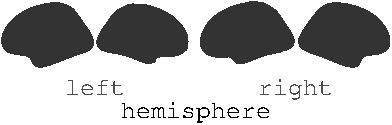
\includegraphics{draft_2_files/figure-latex/init-1.pdf}
\caption{\label{fig:init}By default \texttt{ggseg} will plot the dkt atlas in shaded polygons.}
\end{figure}

\texttt{ggseg} is implemented as a fully-functional part of ggplot.
Thus one should be able to use the function together with any other ggplot function such as themes or scales.
You can stack the hemispheres, view only the medial or lateral side, choose either or both of the hemispheres, or a combination of any of these.
One has several options for plotting the main brain representations.
These options are atlas-specific.
For cortical atlases, such as the `dkt', one can stack the hemispheres, plot one or both hemisphere, or view only the medial or lateral side (or any combination of these; see Figure \ref{fig:collection}).
For subcortical atlases, such as the `aseg', the options are more limited but one can often choose between axial, sagital, and coronal views.

\begin{Shaded}
\begin{Highlighting}[]
\CommentTok{# dkt dark theme}
\NormalTok{p1 <-}\StringTok{ }\KeywordTok{ggseg}\NormalTok{(}\DataTypeTok{position =} \StringTok{"stacked"}\NormalTok{) }\OperatorTok{+}
\StringTok{  }\KeywordTok{theme_dark}\NormalTok{() }\OperatorTok{+}
\StringTok{  }\KeywordTok{labs}\NormalTok{(}\DataTypeTok{title=}\StringTok{" "}\NormalTok{)}

\CommentTok{# dkt classic theme}
\NormalTok{p2 <-}\StringTok{ }\KeywordTok{ggseg}\NormalTok{(}\DataTypeTok{position =} \StringTok{"stacked"}\NormalTok{) }\OperatorTok{+}
\StringTok{  }\KeywordTok{theme_classic}\NormalTok{() }\OperatorTok{+}
\StringTok{  }\KeywordTok{labs}\NormalTok{(}\DataTypeTok{title =} \StringTok{" "}\NormalTok{)}

\CommentTok{# dkt medial view}
\NormalTok{med <-}\StringTok{ }\KeywordTok{ggseg}\NormalTok{(}\DataTypeTok{view =} \StringTok{"medial"}\NormalTok{) }\OperatorTok{+}
\StringTok{  }\KeywordTok{labs}\NormalTok{(}\DataTypeTok{title =} \StringTok{" "}\NormalTok{)}

\CommentTok{# dkt left hemisphere}
\NormalTok{left <-}\StringTok{ }\KeywordTok{ggseg}\NormalTok{(}\DataTypeTok{hemisphere =} \StringTok{"left"}\NormalTok{) }\OperatorTok{+}
\StringTok{  }\KeywordTok{labs}\NormalTok{(}\DataTypeTok{title =} \StringTok{" "}\NormalTok{)}


\CommentTok{# aseg default theme}
\NormalTok{p3 <-}\StringTok{ }\KeywordTok{ggseg}\NormalTok{(}\DataTypeTok{atlas=}\NormalTok{aseg) }\OperatorTok{+}
\StringTok{  }\KeywordTok{labs}\NormalTok{(}\DataTypeTok{title =} \StringTok{" "}\NormalTok{)}


\CommentTok{# dkt left medial alone}
\NormalTok{combo <-}\StringTok{ }\KeywordTok{ggseg}\NormalTok{(}\DataTypeTok{view =} \StringTok{"medial"}\NormalTok{,}
      \DataTypeTok{hemisphere =} \StringTok{"left"}\NormalTok{) }\OperatorTok{+}
\StringTok{  }\KeywordTok{labs}\NormalTok{(}\DataTypeTok{title=}\StringTok{" "}\NormalTok{)}

\CommentTok{# Combine plots}
\NormalTok{cowplot}\OperatorTok{::}\KeywordTok{plot_grid}\NormalTok{(p1, med, combo,  p2, left, p3,}
                   \DataTypeTok{labels =} \KeywordTok{c}\NormalTok{(}\StringTok{"A: dkt - dark"}\NormalTok{, }\StringTok{"B: dkt - medial"}\NormalTok{,}
                              \StringTok{"C: dkt - combo"}\NormalTok{, }\StringTok{"D: dkt - classic"}\NormalTok{,}
                              \StringTok{"E: dkt - left"}\NormalTok{, }\StringTok{"F: aseg"}\NormalTok{),}
                   \DataTypeTok{hjust =} \FloatTok{-.05}\NormalTok{)}
\end{Highlighting}
\end{Shaded}

\begin{figure}
\centering
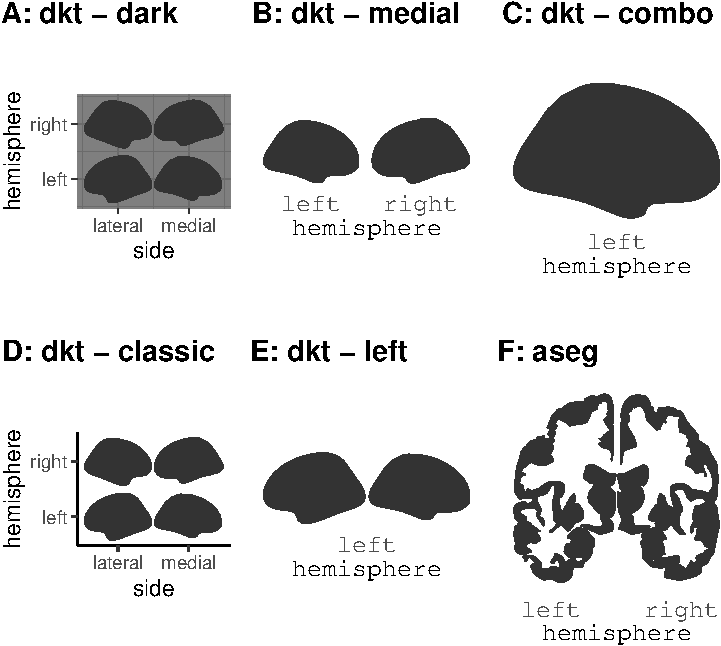
\includegraphics{draft_2_files/figure-latex/collection-1.pdf}
\caption{\label{fig:collection}ggseg plots can be used with most standard scales, themes and such that work with ggplot. The special ggseg options for hemispheres, view etc. depend on the atlas used, and some options are only available for certain atlases. There is no `lateral' or `medial' views of subcortical atlases. There are several ggseg-special options that may be supplied to control how the plots looks and is organised. \textbf{A:} dkt atlas, stacked with dark theme ; \textbf{B:} dkt with medial view only; \textbf{C:} dkt atlas with only left medial display; \textbf{D:} dkt atlas, stacked, with classic theme; \textbf{E:} dkt atlas with left hemisphere only; \textbf{F:} complete aseg atlas}
\end{figure}

\hypertarget{using-own-data-with-fill-and-colour}{%
\subsubsection{Using own data with fill and colour}\label{using-own-data-with-fill-and-colour}}

\texttt{ggseg} accepts any argument you can supply to \texttt{geom\_polygon} and therefore is easy to work with for those familiar with ggplot functionality.
Standard arguments like \texttt{fill} to flood the segments with a colour, or \texttt{colour} to colour the edges around the segments are typical arguments to provide to the function either as a single value or within the ggplot mapping option \texttt{aes}.
To use color palettes corresponding to those used in the original neuroimaging softwares one can use atlas-specific `brain' palette scales.
See an example in Figure \ref{fig:fill}.

\begin{Shaded}
\begin{Highlighting}[]
\KeywordTok{ggseg}\NormalTok{(}\DataTypeTok{mapping=}\KeywordTok{aes}\NormalTok{(}\DataTypeTok{fill =}\NormalTok{ area), }\DataTypeTok{colour=}\StringTok{"black"}\NormalTok{) }\OperatorTok{+}
\StringTok{  }\KeywordTok{scale_fill_brain}\NormalTok{(}\StringTok{"dkt"}\NormalTok{) }\OperatorTok{+}
\StringTok{  }\KeywordTok{theme}\NormalTok{(}\DataTypeTok{legend.justification=}\KeywordTok{c}\NormalTok{(}\DecValTok{1}\NormalTok{,}\DecValTok{0}\NormalTok{),}
        \DataTypeTok{legend.position=}\StringTok{"bottom"}\NormalTok{,}
        \DataTypeTok{legend.text =} \KeywordTok{element_text}\NormalTok{(}\DataTypeTok{size =} \DecValTok{5}\NormalTok{)) }\OperatorTok{+}
\StringTok{  }\KeywordTok{guides}\NormalTok{(}\DataTypeTok{fill =} \KeywordTok{guide_legend}\NormalTok{(}\DataTypeTok{ncol =} \DecValTok{3}\NormalTok{))}
\end{Highlighting}
\end{Shaded}

\begin{figure}
\centering
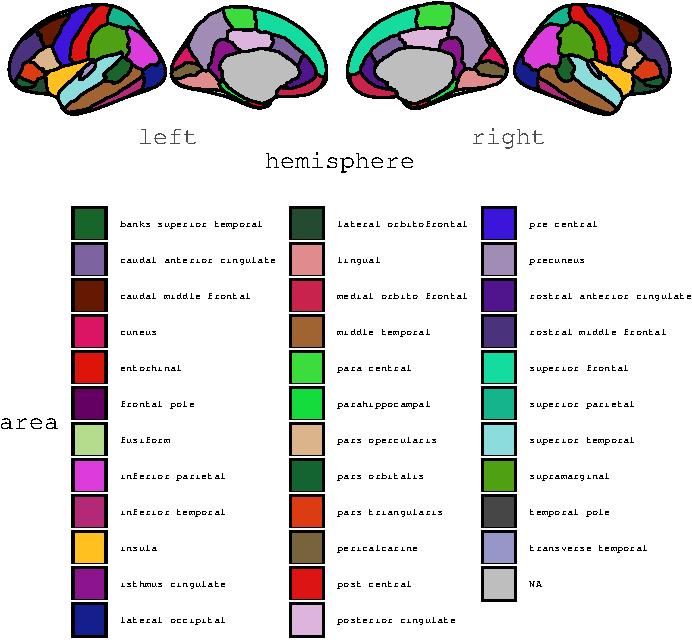
\includegraphics{draft_2_files/figure-latex/fill-1.pdf}
\caption{\label{fig:fill}Supplying `area' to the fill option in ggseg, will use the column `area' from the accompanying dataset to create a discrete colour palette over the segments in the atlas.}
\end{figure}

Most users will use ggseg to display - using a color scale - some descriptive or inferential statistics, such as mean thickness or cognition relationships etc., across the different brain regions.
The bulk of the package originates not in its functions, but in the data sets that accompany the package.
There is one data set per atlas, which contains key information regarding the atlas, and coordinates for the segment polygons of the atlas.
Before setting up the data from the statistics to project onto the segments, looking at the atlas data sets might help understand what the data needs to look like, or avoid looking like.

\small

\begin{Shaded}
\begin{Highlighting}[]
\NormalTok{dkt}
\end{Highlighting}
\end{Shaded}

\begin{verbatim}
## # A tibble: 80 x 6
##    atlas area               hemi  side    label             ggseg          
##    <chr> <chr>              <chr> <chr>   <chr>             <list>         
##  1 dkt   superior temporal  left  lateral lh_superiortempo~ <tibble [1,494~
##  2 dkt   pre central        left  lateral lh_precentral     <tibble [1,314~
##  3 dkt   post central       left  lateral lh_postcentral    <tibble [1,164~
##  4 dkt   rostral middle fr~ left  lateral lh_rostralmiddle~ <tibble [1,194~
##  5 dkt   insula             left  lateral lh_insula         <tibble [870 x~
##  6 dkt   superior parietal  left  lateral lh_superiorparie~ <tibble [480 x~
##  7 dkt   inferior temporal  left  lateral lh_inferiortempo~ <tibble [906 x~
##  8 dkt   lateral occipital  left  lateral lh_lateraloccipi~ <tibble [738 x~
##  9 dkt   lateral orbitofro~ left  lateral lh_lateralorbito~ <tibble [528 x~
## 10 dkt   superior frontal   left  lateral lh_superiorfront~ <tibble [420 x~
## # ... with 70 more rows
\end{verbatim}

\normalsize

In any atlas, the column `label' is particularly useful for combining the data of interest with the \texttt{ggseg}-polygons.
The column `label' contains the label (region) names as in the original neuroimaging software.
For example, the DKT atlas label column matches the region names from Freesurfer statistics tables.
Yet the data in \texttt{ggseg} is in a long format - that is each region has its own row - and data of interest needs to be in this same format.
Most data sets are organized in wide format, in which subjects are represented by rows and each different data variable is represented in a separate column, and thus need to be rearranged in order to work with ggseg.
See below an example of wide-to-long conversion.

\begin{Shaded}
\begin{Highlighting}[]
\NormalTok{freesurfer_stats <-}\StringTok{ }\KeywordTok{data.frame}\NormalTok{(}
  \DataTypeTok{id =} \KeywordTok{c}\NormalTok{(}\DecValTok{10}\OperatorTok{:}\DecValTok{12}\NormalTok{),}
  \DataTypeTok{lh_superiortemporal =} \KeywordTok{c}\NormalTok{(}\FloatTok{3.32}\NormalTok{, }\FloatTok{4.1}\NormalTok{, }\FloatTok{3.5}\NormalTok{),}
  \DataTypeTok{lh_precentral =} \KeywordTok{c}\NormalTok{(}\FloatTok{2.3}\NormalTok{, }\FloatTok{2.5}\NormalTok{, }\FloatTok{2.1}\NormalTok{),}
  \DataTypeTok{lh_rostralmiddlefrontal =} \KeywordTok{c}\NormalTok{(}\FloatTok{3.3}\NormalTok{, }\FloatTok{3.2}\NormalTok{, }\FloatTok{3.1}\NormalTok{)}
\NormalTok{  )}
\NormalTok{freesurfer_stats}
\end{Highlighting}
\end{Shaded}

\begin{verbatim}
##   id lh_superiortemporal lh_precentral lh_rostralmiddlefrontal
## 1 10                3.32           2.3                     3.3
## 2 11                4.10           2.5                     3.2
## 3 12                3.50           2.1                     3.1
\end{verbatim}

\begin{Shaded}
\begin{Highlighting}[]
\NormalTok{freesurfer_long <-}\StringTok{ }\NormalTok{freesurfer_stats }\OperatorTok
\StringTok{  }\KeywordTok{gather}\NormalTok{(label, thickness, }\OperatorTok{-}\NormalTok{id)}
\NormalTok{freesurfer_long}
\end{Highlighting}
\end{Shaded}

\begin{verbatim}
##   id                   label thickness
## 1 10     lh_superiortemporal      3.32
## 2 11     lh_superiortemporal      4.10
## 3 12     lh_superiortemporal      3.50
## 4 10           lh_precentral      2.30
## 5 11           lh_precentral      2.50
## 6 12           lh_precentral      2.10
## 7 10 lh_rostralmiddlefrontal      3.30
## 8 11 lh_rostralmiddlefrontal      3.20
## 9 12 lh_rostralmiddlefrontal      3.10
\end{verbatim}

This data - in long format - can now be used directly with the \texttt{ggseg} function, as the \texttt{label} column corresponds in name and content with the \texttt{label} column in the atlas data of dkt.
The data \textbf{must} include a column that has the same name and at least \emph{some} data matching the values in the corresponding column in the atlas data.
In the next example we create some data with 4 rows, and an `area' and `p' column, representing the results of an analysis.
The \texttt{ggseg} function will recognise the matching column `area', and merge the supplied data into the atlas using \texttt{dplyr} joins.
We use the \texttt{p} column as the column flooding the segment with colour.

\begin{Shaded}
\begin{Highlighting}[]
\NormalTok{someData =}\StringTok{ }\KeywordTok{data.frame}\NormalTok{(}
  \DataTypeTok{area =} \KeywordTok{c}\NormalTok{(}\StringTok{"transverse temporal"}\NormalTok{, }\StringTok{"insula"}\NormalTok{,}
           \StringTok{"pre central"}\NormalTok{,}\StringTok{"superior parietal"}\NormalTok{),}
  \DataTypeTok{p =} \KeywordTok{sample}\NormalTok{(}\KeywordTok{seq}\NormalTok{(}\DecValTok{0}\NormalTok{,.}\DecValTok{5}\NormalTok{,.}\DecValTok{001}\NormalTok{), }\DecValTok{4}\NormalTok{),}
  \DataTypeTok{stringsAsFactors =} \OtherTok{FALSE}\NormalTok{)}

\NormalTok{p <-}\StringTok{ }\KeywordTok{ggseg}\NormalTok{(}\DataTypeTok{.data=}\NormalTok{someData, }\DataTypeTok{mapping=}\KeywordTok{aes}\NormalTok{(}\DataTypeTok{fill=}\NormalTok{p))}
\NormalTok{p}
\end{Highlighting}
\end{Shaded}

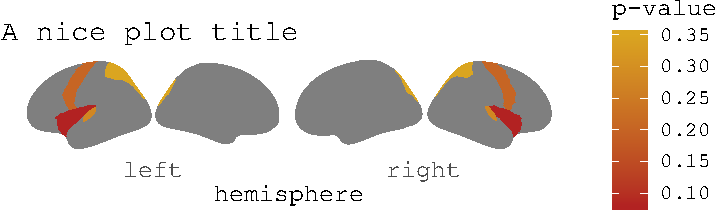
\includegraphics{draft_2_files/figure-latex/datasupp-1.pdf}

The appearance of this plot can then be modified similarly to any other ggplot graph using functions such as scales, labs, themes, etc.

\begin{Shaded}
\begin{Highlighting}[]
\NormalTok{p }\OperatorTok{+}
\StringTok{  }\KeywordTok{theme_void}\NormalTok{() }\OperatorTok{+}
\StringTok{  }\KeywordTok{scale_fill_gradient}\NormalTok{(}\DataTypeTok{low=}\StringTok{"firebrick"}\NormalTok{,}\DataTypeTok{high=}\StringTok{"goldenrod"}\NormalTok{) }\OperatorTok{+}
\StringTok{  }\KeywordTok{labs}\NormalTok{(}\DataTypeTok{title=}\StringTok{"A nice plot title"}\NormalTok{, }\DataTypeTok{fill=}\StringTok{"p-value"}\NormalTok{)}
\end{Highlighting}
\end{Shaded}

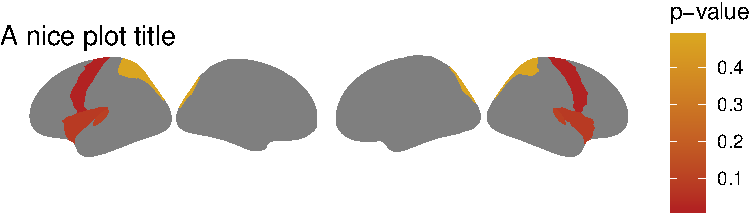
\includegraphics{draft_2_files/figure-latex/datasupp2-1.pdf}

If the results are only in one hemisphere, but you still want to plot both of them, make sure your data.fame includes the column \texttt{hemi} with either `right' or `left' for this to happen.

\begin{Shaded}
\begin{Highlighting}[]
\NormalTok{someData}\OperatorTok{$}\NormalTok{hemi =}\StringTok{ "right"}

\KeywordTok{ggseg}\NormalTok{(}\DataTypeTok{.data=}\NormalTok{someData, }\DataTypeTok{colour=}\StringTok{"white"}\NormalTok{,}\DataTypeTok{mapping=}\KeywordTok{aes}\NormalTok{(}\DataTypeTok{fill=}\NormalTok{p)) }\OperatorTok{+}
\StringTok{  }\KeywordTok{theme_void}\NormalTok{() }\OperatorTok{+}
\StringTok{  }\KeywordTok{scale_fill_gradient}\NormalTok{(}\DataTypeTok{low=}\StringTok{"firebrick"}\NormalTok{,}\DataTypeTok{high=}\StringTok{"goldenrod"}\NormalTok{) }\OperatorTok{+}
\StringTok{  }\KeywordTok{labs}\NormalTok{(}\DataTypeTok{title=}\StringTok{"Another nice plot title"}\NormalTok{)}
\end{Highlighting}
\end{Shaded}

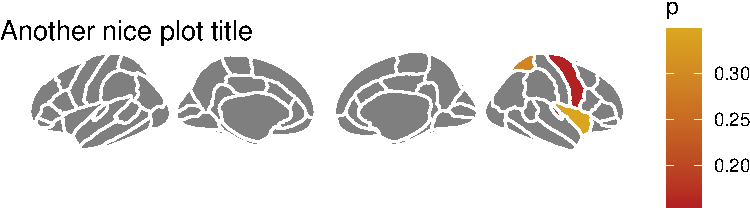
\includegraphics{draft_2_files/figure-latex/datasuppX-1.pdf}

\hypertarget{creating-subplots}{%
\subsubsection{Creating subplots}\label{creating-subplots}}

There is often the need to plot a statistic of interest in different groups (i.e.~thickness or significance in young or older adults).
This may be obtained also with ggseg, using ggplot's \texttt{facet\_wrap} or \texttt{facet\_grid}, using two guiding rules:
\textbf{1)} as before, data needs to be in long format (group data should appear in seperate rows, not in separate columns).
\textbf{2)} The data needs to be grouped using \texttt{dplyr}'s \texttt{group\_by} function \emph{before} providing the data to the \texttt{ggseg} function.
The ggseg function will detect grouped data, and adapt it to \texttt{facet}'s requirements.

\begin{Shaded}
\begin{Highlighting}[]
\NormalTok{someData =}\StringTok{ }\KeywordTok{data.frame}\NormalTok{(}
  \DataTypeTok{area =} \KeywordTok{rep}\NormalTok{(}\KeywordTok{c}\NormalTok{(}\StringTok{"transverse temporal"}\NormalTok{, }\StringTok{"insula"}\NormalTok{,}
               \StringTok{"pre central"}\NormalTok{,}\StringTok{"superior parietal"}\NormalTok{),}\DecValTok{2}\NormalTok{),}
  \DataTypeTok{p =} \KeywordTok{sample}\NormalTok{(}\KeywordTok{seq}\NormalTok{(}\DecValTok{0}\NormalTok{,.}\DecValTok{5}\NormalTok{,.}\DecValTok{001}\NormalTok{), }\DecValTok{8}\NormalTok{),}
  \DataTypeTok{AgeG =} \KeywordTok{c}\NormalTok{(}\KeywordTok{rep}\NormalTok{(}\StringTok{"Young"}\NormalTok{,}\DecValTok{4}\NormalTok{), }\KeywordTok{rep}\NormalTok{(}\StringTok{"Old"}\NormalTok{,}\DecValTok{4}\NormalTok{)),}
  \DataTypeTok{stringsAsFactors =} \OtherTok{FALSE}\NormalTok{) }\OperatorTok
\StringTok{  }\KeywordTok{group_by}\NormalTok{(AgeG)}

\KeywordTok{ggseg}\NormalTok{(}\DataTypeTok{.data=}\NormalTok{someData, }\DataTypeTok{colour=}\StringTok{"white"}\NormalTok{, }\DataTypeTok{mapping=}\KeywordTok{aes}\NormalTok{(}\DataTypeTok{fill=}\NormalTok{p)) }\OperatorTok{+}
\StringTok{  }\KeywordTok{facet_wrap}\NormalTok{(}\OperatorTok{~}\NormalTok{AgeG, }\DataTypeTok{ncol=}\DecValTok{1}\NormalTok{) }\OperatorTok{+}
\StringTok{  }\KeywordTok{theme}\NormalTok{(}\DataTypeTok{legend.position =} \StringTok{"bottom"}\NormalTok{)}
\end{Highlighting}
\end{Shaded}

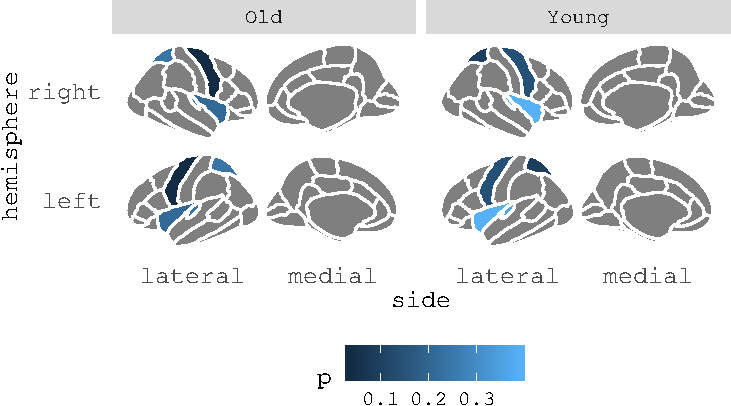
\includegraphics{draft_2_files/figure-latex/datasupp3-1.pdf}

As before, one can apply the different ggplot and facet options, such as \texttt{scales} to modify the plot's appearance.

\begin{Shaded}
\begin{Highlighting}[]
\KeywordTok{ggseg}\NormalTok{(}\DataTypeTok{.data =}\NormalTok{ someData, }\DataTypeTok{atlas=}\NormalTok{dkt,}
      \DataTypeTok{colour=}\StringTok{"white"}\NormalTok{, }\DataTypeTok{position=}\StringTok{"stacked"}\NormalTok{,}
      \DataTypeTok{mapping=}\KeywordTok{aes}\NormalTok{(}\DataTypeTok{fill=}\NormalTok{p)) }\OperatorTok{+}
\StringTok{  }\KeywordTok{facet_wrap}\NormalTok{(}\OperatorTok{~}\NormalTok{AgeG, }\DataTypeTok{ncol=}\DecValTok{2}\NormalTok{) }\OperatorTok{+}
\StringTok{  }\KeywordTok{theme_dark}\NormalTok{() }\OperatorTok{+}
\StringTok{  }\KeywordTok{theme}\NormalTok{(}\DataTypeTok{legend.position =} \StringTok{"bottom"}\NormalTok{,}
        \DataTypeTok{axis.text =} \KeywordTok{element_blank}\NormalTok{(),}
        \DataTypeTok{axis.title =} \KeywordTok{element_blank}\NormalTok{()}
\NormalTok{        ) }\OperatorTok{+}
\StringTok{  }\KeywordTok{scale_fill_gradient2}\NormalTok{(}\DataTypeTok{high=}\StringTok{"goldenrod"}\NormalTok{,}
                       \DataTypeTok{low=}\StringTok{"firebrick"}\NormalTok{,}
                       \DataTypeTok{na.value=}\StringTok{"transparent"}\NormalTok{)}
\end{Highlighting}
\end{Shaded}

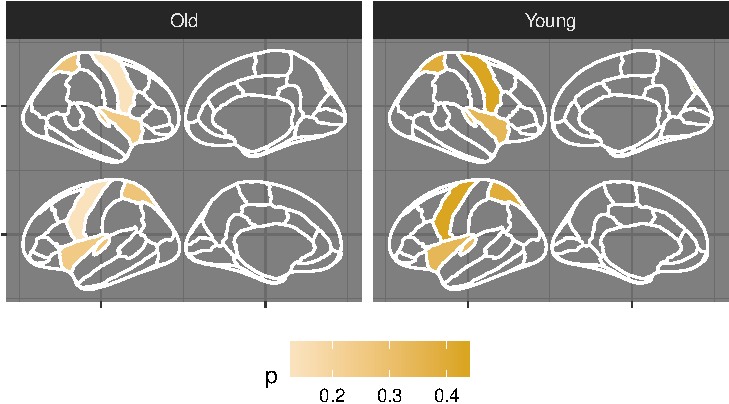
\includegraphics{draft_2_files/figure-latex/datasupp5-1.pdf}

All the concepts described above also work with the `aseg' atlas for subcortical structures, except hemisphere and view arguments that do not apply in the same way in subcortical atlases such as aseg.
Again, inspecting the atlas data directly will be of aid when preparing data to use with the atlas.

\small

\begin{Shaded}
\begin{Highlighting}[]
\NormalTok{aseg}
\end{Highlighting}
\end{Shaded}

\begin{verbatim}
## # A tibble: 34 x 6
##    atlas area            hemi  side  label                ggseg            
##    <chr> <chr>           <chr> <chr> <fct>                <list>           
##  1 aseg  <NA>            right axial <NA>                 <tibble [808 x 5~
##  2 aseg  <NA>            left  axial <NA>                 <tibble [1,014 x~
##  3 aseg  thalamus proper left  axial Left-Thalamus-Proper <tibble [56 x 5]>
##  4 aseg  thalamus proper left  axial Right-Thalamus-Prop~ <tibble [56 x 5]>
##  5 aseg  thalamus proper right axial Left-Thalamus-Proper <tibble [61 x 5]>
##  6 aseg  thalamus proper right axial Right-Thalamus-Prop~ <tibble [61 x 5]>
##  7 aseg  lateral ventri~ right axial Left-Lateral-Ventri~ <tibble [66 x 5]>
##  8 aseg  lateral ventri~ right axial Right-Lateral-Ventr~ <tibble [66 x 5]>
##  9 aseg  hippocampus     left  axial Left-Hippocampus     <tibble [47 x 5]>
## 10 aseg  hippocampus     left  axial Right-Hippocampus    <tibble [47 x 5]>
## # ... with 24 more rows
\end{verbatim}

\normalsize

\begin{Shaded}
\begin{Highlighting}[]
\KeywordTok{ggseg}\NormalTok{(}\DataTypeTok{atlas=}\StringTok{"aseg"}\NormalTok{, }\DataTypeTok{mapping=}\KeywordTok{aes}\NormalTok{(}\DataTypeTok{fill=}\NormalTok{area))}
\end{Highlighting}
\end{Shaded}

\begin{figure}
\centering
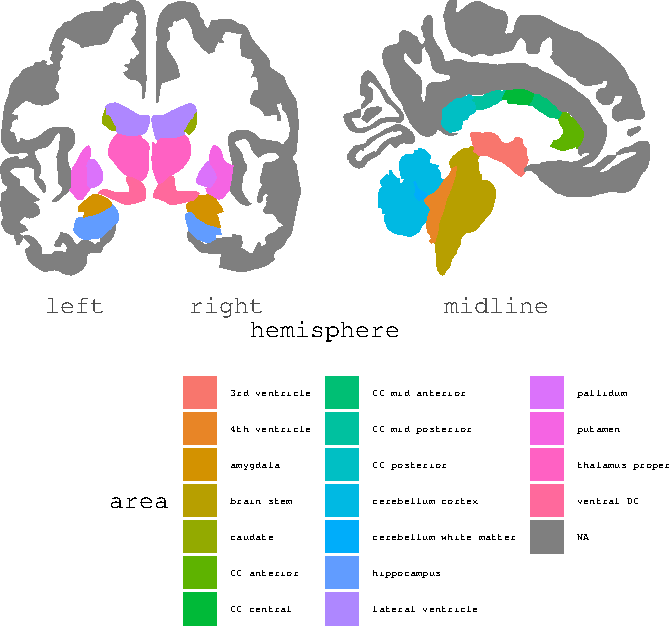
\includegraphics{draft_2_files/figure-latex/atlases-1.pdf}
\caption{\label{fig:atlases}The first 10 rows of the \texttt{aseg} dataset, that has some specific differences from the dkt, like missing the option to not view both hemispheres, as the plot would be hard to understand that way.}
\end{figure}

\hypertarget{plotting-3d-mesh-data}{%
\subsection{Plotting 3D mesh data}\label{plotting-3d-mesh-data}}

Representing brains as 2D polygons is a good solution for fast, efficient, and flexible plotting, and can be easily combined with interactive apps such as Shiny (\citet{shiny}).
Yet, brains are intrinsically 3-dimensional and it can be challenging to recognize the location of a region as a flattened image.
This problem is exacerbated in atlases that represent subcortical features -- after all, cortical surfaces are 2-dimensional -- such as grey matter structures or white matter tracts.
Hence, here we also provide the \texttt{ggseg3d} function to plot, view, and print 3D-atlases in R.
\texttt{ggseg3d} is based on tri-surface mesh plots using plotly (\citet{plotly}).
The data structure is somewhat more complex than the ggplot polygons, and includes additional options for brain inflation, glass brains, camera locations, etc.
As \texttt{ggseg3d} is based on plotly, the resulting brain atlases are interactive, which guides interpretation, and is useful for public dissemination.
We recommend users to familiarize themselves with plotly (\citet{plotly}) when using this function.

Out-of-the-box, \texttt{ggseg3d()} plots the \texttt{dkt\_3d} atlas in `LCBC' surface.
The `LCBC' surface consists on a semi-inflated white matter surface based on the \emph{fsaverage} template subject.
See \emph{SI SCRIPT} for reproducibility.
All \texttt{{[}...{]}\_3d} atlases have a built in \texttt{colour} column for default colour plotting of the regions, based on the colorlut used in the neuroimaging software.

\begin{figure}
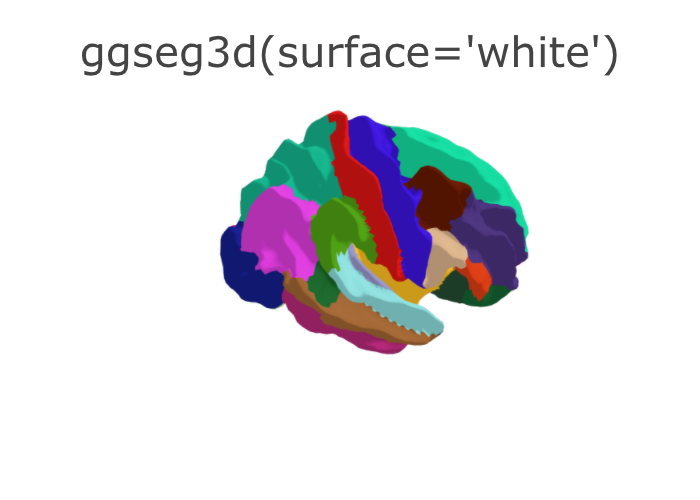
\includegraphics[width=0.3\linewidth]{png/ggseg3d_white} 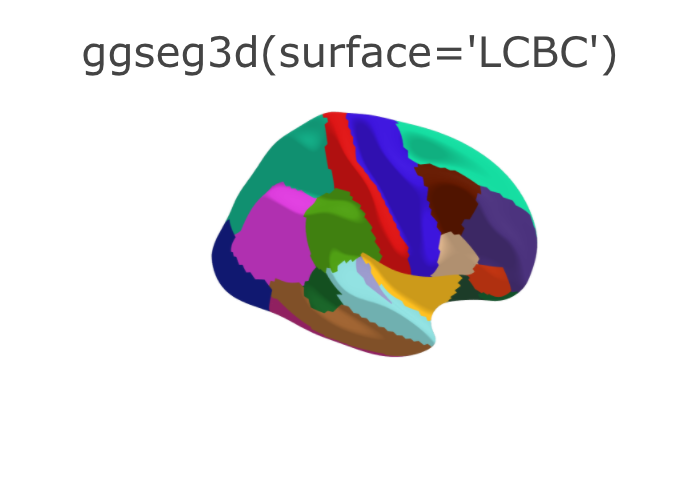
\includegraphics[width=0.3\linewidth]{png/ggseg3d} 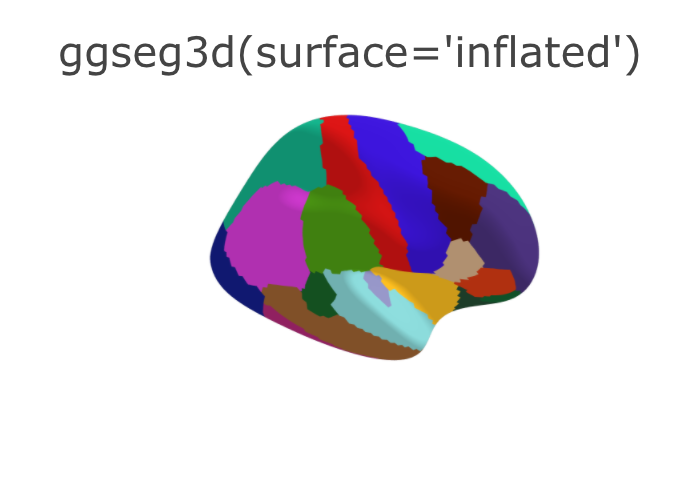
\includegraphics[width=0.3\linewidth]{png/ggseg3d_inflated} \caption{The three surface options provided in ggseg 3d atlases. From left: the 'white' surface is the white matter surface, 'LCBC' surface is the white matter surface inflated in 10 steps, and the 'inflated' surface is a fully inflated sortical surface.}\label{fig:ggseg3d-1-out}
\end{figure}

The 3D-atlas data is stored in nested tibbles.
Each cortical atlas has data sets for three different surfaces (see Figure @ref(fig:ggseg3d\_1\_out)) and the two hemispheres.
As there are no meaningful other surfaces for subcortical atlases, these only have a single surface.
The `ggseg\_3d' column includes all necessary information to \texttt{ggseg3d()} to create a mesh-plot.
The additional 3D-atlases in ggsegExtra have the same data structure.

\small

\begin{Shaded}
\begin{Highlighting}[]
\NormalTok{dkt_3d}
\end{Highlighting}
\end{Shaded}

\begin{verbatim}
## # A tibble: 6 x 4
##   atlas  surf     hemi  ggseg_3d         
##   <chr>  <chr>    <chr> <list>           
## 1 dkt_3d inflated left  <tibble [36 x 8]>
## 2 dkt_3d inflated right <tibble [36 x 8]>
## 3 dkt_3d LCBC     left  <tibble [36 x 8]>
## 4 dkt_3d LCBC     right <tibble [36 x 8]>
## 5 dkt_3d white    left  <tibble [36 x 8]>
## 6 dkt_3d white    right <tibble [36 x 8]>
\end{verbatim}

\normalsize

\hypertarget{external-data-supply}{%
\subsubsection{External data supply}\label{external-data-supply}}

Similarly as in the 2D-atlas, the user will use \texttt{ggseg3d} to display through a color scale some descriptive or inferential statistics.
If the data is not already in the correct long format, or uses similar naming as the atlas, one needs to grab the data for a specific surface (and hemisphere, if desired) and then \texttt{unnest(ggseg\_3d)} it to see what the atlas is expecting.

\begin{Shaded}
\begin{Highlighting}[]
\NormalTok{dkt_3d }\OperatorTok
\StringTok{  }\KeywordTok{filter}\NormalTok{(surf }\OperatorTok{==}\StringTok{ "inflated"} \OperatorTok{&}\StringTok{ }\NormalTok{hemi }\OperatorTok{==}\StringTok{ "right"}\NormalTok{) }\OperatorTok
\StringTok{  }\KeywordTok{unnest}\NormalTok{(ggseg_3d) }\OperatorTok
\StringTok{  }\KeywordTok{select}\NormalTok{(}\OperatorTok{-}\NormalTok{lobe, }\OperatorTok{-}\NormalTok{acronym)}
\end{Highlighting}
\end{Shaded}

\begin{verbatim}
## # A tibble: 36 x 9
## atlas surf hemi area colour mesh label roi annot
## <chr> <chr> <chr> <chr> <chr> <list> <chr> <chr> <chr>
## 1 dkt_3d infla~ right <NA> <NA> <list~ rh_medial~ 0001 medialwa~
## 2 dkt_3d infla~ right banks supe~ #1964~ <list~ rh_bankss~ 0002
bankssts
## 3 dkt_3d infla~ right caudal ant~ #7D64~ <list~ rh_caudal~ 0003
caudalan~
## 4 dkt_3d infla~ right caudal mid~ #6419~ <list~ rh_caudal~ 0004
caudalmi~
## 5 dkt_3d infla~ right corpus cal~ <NA> <list~ rh_corpus~ 0005
corpusca~
## 6 dkt_3d infla~ right cuneus #DC14~ <list~ rh_cuneus 0006 cuneus
## 7 dkt_3d infla~ right entorhinal #DC14~ <list~ rh_entorh~ 0007
entorhin~
## 8 dkt_3d infla~ right fusiform #B4DC~ <list~ rh_fusifo~ 0008
fusiform
## 9 dkt_3d infla~ right inferior p~ #DC3C~ <list~ rh_inferi~ 0009
inferior~
## 10 dkt_3d infla~ right inferior t~ #B428~ <list~ rh_inferi~ 0010
inferior~
## # ... with 26 more rows
\end{verbatim}

Note the \texttt{mesh} column, which contains lists.
Each list corresponds to a region and contains 6 vectors required to create the mesh of the tri-surface plot.
It should also be noted that the `label', `annot' and `area' columns could provide matching values for your own data.
Similarly to the \texttt{ggseg}-function, the `label' column should match the region names used in the original neuroimaging software while `area' and `annot' provide alternative/secondary names.
It is thus important to match your regional identifiers with those used in the atlas.
A warning will be issued in case of any mismatch.
The column you want to use for colour, needs to be supplied to the \texttt{colour} option, and you'll likely want to supply it to the \texttt{text} option, as this will add another line to the plotly hover information.

\begin{Shaded}
\begin{Highlighting}[]
\NormalTok{someData =}\StringTok{ }\NormalTok{dkt_3d }\OperatorTok
\StringTok{  }\KeywordTok{filter}\NormalTok{(surf }\OperatorTok{==}\StringTok{ "inflated"} \OperatorTok{&}
\StringTok{         }\NormalTok{hemi }\OperatorTok{==}\StringTok{ "right"}\NormalTok{) }\OperatorTok
\StringTok{  }\KeywordTok{unnest}\NormalTok{(ggseg_3d) }\OperatorTok
\StringTok{  }\KeywordTok{select}\NormalTok{(area) }\OperatorTok
\StringTok{  }\KeywordTok{na.omit}\NormalTok{() }\OperatorTok
\StringTok{  }\KeywordTok{mutate}\NormalTok{(}\DataTypeTok{p =} \KeywordTok{sample}\NormalTok{(}\KeywordTok{seq}\NormalTok{(}\DecValTok{0}\NormalTok{,.}\DecValTok{5}\NormalTok{, }\DataTypeTok{length.out =} \DecValTok{100}\NormalTok{ ), }\KeywordTok{nrow}\NormalTok{(.)) }\OperatorTok
\StringTok{           }\KeywordTok{round}\NormalTok{(}\DecValTok{2}\NormalTok{))}

  \KeywordTok{ggseg3d}\NormalTok{(}\DataTypeTok{.data =}\NormalTok{ someData, }\DataTypeTok{atlas =}\NormalTok{ dkt_3d, }\DataTypeTok{colour =} \StringTok{"p"}\NormalTok{, }\DataTypeTok{text =} \StringTok{"p"}\NormalTok{)}
\end{Highlighting}
\end{Shaded}

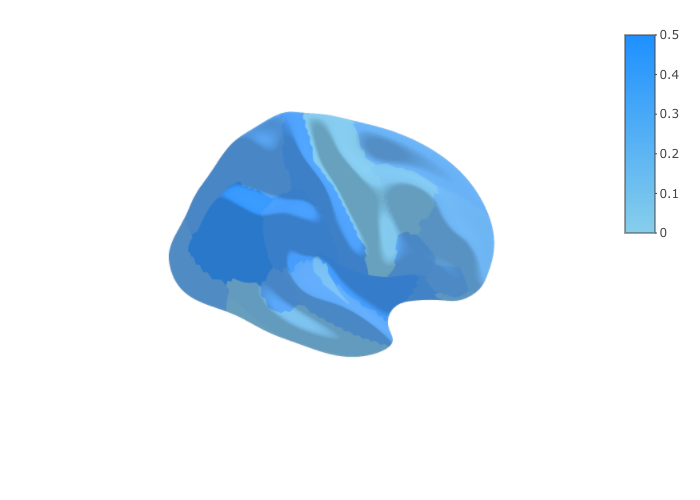
\includegraphics[width=0.4\linewidth]{png/ggseg3d_data}

\hypertarget{colours}{%
\subsubsection{Colours}\label{colours}}

You can provide custom colour palettes either in hex or R-names.
Colours will be evenly spaced when creating the colour-scale, and you may provide as many colours as you wish.

\begin{Shaded}
\begin{Highlighting}[]
  \KeywordTok{ggseg3d}\NormalTok{(}\DataTypeTok{.data =}\NormalTok{ someData, }\DataTypeTok{atlas =}\NormalTok{ dkt_3d,}
          \DataTypeTok{colour =} \StringTok{"p"}\NormalTok{, }\DataTypeTok{text =} \StringTok{"p"}\NormalTok{,}
          \DataTypeTok{palette =} \KeywordTok{c}\NormalTok{(}\StringTok{"#ff0000"}\NormalTok{, }\StringTok{"#00ff00"}\NormalTok{, }\StringTok{"#0000ff"}\NormalTok{))}
\end{Highlighting}
\end{Shaded}

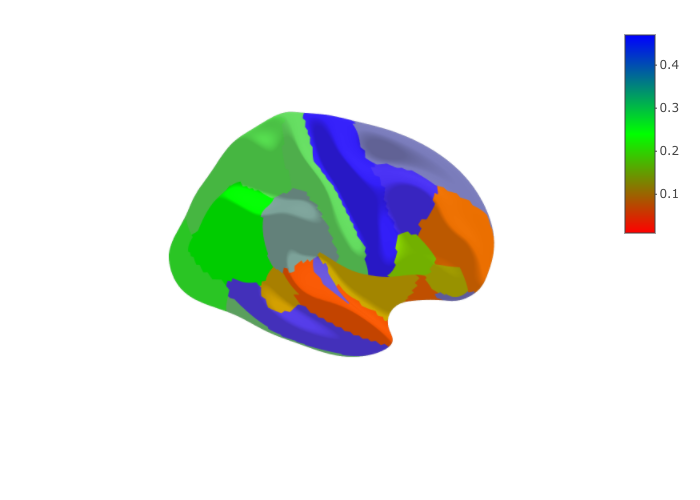
\includegraphics[width=0.4\linewidth]{png/ggseg3d_colour}

If you want to alter the colour of \texttt{NA} regions, supply \texttt{na.colour}, either as HEX colour or colour name.
This option only takes a single colour.

\begin{Shaded}
\begin{Highlighting}[]
  \KeywordTok{ggseg3d}\NormalTok{(}\DataTypeTok{.data =}\NormalTok{ someData, }\DataTypeTok{atlas =}\NormalTok{ dkt_3d,}
          \DataTypeTok{colour =} \StringTok{"p"}\NormalTok{, }\DataTypeTok{text =} \StringTok{"p"}\NormalTok{,}
          \DataTypeTok{na.colour =} \StringTok{"black"}\NormalTok{, }\DataTypeTok{camera=}\StringTok{"medial"}\NormalTok{)}
\end{Highlighting}
\end{Shaded}

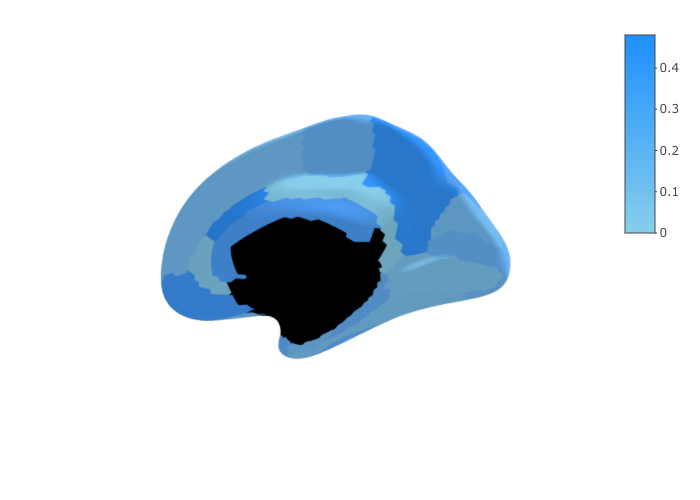
\includegraphics[width=0.4\linewidth]{png/ggseg3d_nacolour}

Subcortical atlases include cortical surfaces and other landmark structures for visualization purposes only.
One can control the opacity of the these \texttt{NA} structures, to improve visualization.
Additionally, one can add the \texttt{glassbrain} option, which provides a frame of reference for the subcortical structures.
Glassbrains can be controlled with three different arguments: opacity (0-1), hemisphere (left, right), and colour.

\begin{Shaded}
\begin{Highlighting}[]
\NormalTok{somData_aseg =}\StringTok{ }\NormalTok{aseg_3d }\OperatorTok
\StringTok{  }\KeywordTok{unnest}\NormalTok{() }\OperatorTok
\StringTok{  }\KeywordTok{select}\NormalTok{(label) }\OperatorTok
\StringTok{  }\KeywordTok{filter}\NormalTok{(}\OperatorTok{!}\KeywordTok{grepl}\NormalTok{(}\StringTok{"Ventricle|Putamen"}\NormalTok{, label)) }\OperatorTok
\StringTok{  }\KeywordTok{mutate}\NormalTok{(}\DataTypeTok{p =} \KeywordTok{seq}\NormalTok{(}\DecValTok{1}\NormalTok{, }\KeywordTok{nrow}\NormalTok{(.)))}

  \KeywordTok{ggseg3d}\NormalTok{(}\DataTypeTok{.data =}\NormalTok{ somData_aseg, }\DataTypeTok{atlas =}\NormalTok{ aseg_3d,}
          \DataTypeTok{colour =} \StringTok{"p"}\NormalTok{, }\DataTypeTok{text =} \StringTok{"p"}\NormalTok{,}
          \DataTypeTok{na.alpha=} \FloatTok{.5}\NormalTok{, }\DataTypeTok{glassbrain =} \FloatTok{.5}\NormalTok{,}
          \DataTypeTok{glassbrain_hemisphere =} \StringTok{"left"}\NormalTok{)}
\end{Highlighting}
\end{Shaded}

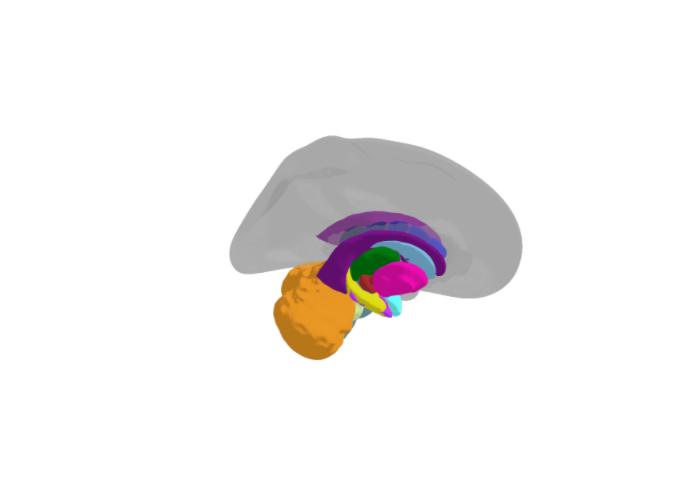
\includegraphics[width=0.4\linewidth]{png/ggseg3d_glass}

\texttt{ggsed3d()} is based on plotly and thus additional plotly functionalities can be used to modify and improve the 3D atlas representations.
In addition to Carson Sievert's book on plotly in R (\citeyearpar{plotly}), we recommend resources for modifying axes in 3D plots (\citet{plotly-ax}), the basic introduction to tri-surface plots (\citet{plotly-tri}), and this tutorial on tri-surface plots with plotly in R (\citet{plotly-trisurf}).
Finally, we recommend \href{https://github.com/plotly/orca\#installation}{orca} command line tool to save ggseg3d atlas snapshots.

\hypertarget{discussion}{%
\section{Discussion}\label{discussion}}

The main aim of the ggseg -- and ggsegExtra - package is to ease and streamline visualization of brain atlas data in R, by gathering a collection of atlases from several scientific sources and providing plotting functions adapted to these atlases.
In this tutorial, we introduce the package to the readers by presenting some use examples and highlighting the main functions and options that are available.
As a visualization tool, this package adds up to manifold functionalities such as ggBrain (\citet{ggBrain}) and ggneuro (\citet{ggneuro}) in R, and software-specific image viewers such as FSLeyes (\citet{fsleyes}) and Freeview (\citet{dale_99}).
In this regard, we do not aim to compete with software-specific visualizations or advocate for the superiority of ggseg as a visualization tool.
After all, flattened 2D polygons do not rely on a meaningful brain coordinate system and the units of information in 3D meshes are limited to the number of parcellations.
On the contrary, we believe the ggseg niche among visualization tools resides in its simplicity and its ability to be combined with statistical analysis pipelines.
The possibility to serve as an interactive tool for dissemination and reproducibility when combined with other technologies, such as Binder (\citet{binder}) or Shiny (\citet{shiny}), is an added benefit.

The ggseg and ggsegExtra packages contain three main features:
\textbf{1)} a collection of 2D-polygon and 3D mesh brain parcellation atlases. The atlas data are necessary to create the coordinate system for the brain atlas plotting, but are made in such a way to make i easy to use for ones own purposes.
\textbf{2)} \texttt{ggseg()} and \texttt{ggseg3d()} functions for visualization.
\texttt{ggseg()} as a wrapper for \texttt{geom\_polygon} from \texttt{ggplot2} and it can be built upon like any ggplot object.
\texttt{ggseg3d()} as a plotly wrapper for tri-surface mesh plots which prints 3D atlases.
Both functions are flexible and well-adapted to its environment as can be combined with any additional argument from ggplot and plotly, respectively.
\textbf{3)} Complimentary features -- e.g.~color scales - and functions such as \texttt{as\_ggseg\_atlas()} and \texttt{as\_ggseg3d\_atlas()} to convert data in the correct atlas format. These function should provide users with the possibility of adapting their plots to their wishes, and also to make it possible to create and contribute to the atlas repository.

The foundations of the ggseg-package trace back to the necessity of visualizing and exploring the lifespan trajectories of cortical thickness across different brain regions (see supporting information in Vidal-Piñeiro et al. (\citeyearpar{vidal_2019})) .
That is, ggseg appears with the need to inspect and display 4D information - including a spatial dimension - overcoming the constrains of printed journals and classical 2D plots (e.g.~bar plots).
The current state of science requires researches to share the results of studies in both high detail and in an intuitive manner, as it permits communication to wide audiences and facilitates reproducibility.
Hence, we believe this tool conforms to the essence of open science and invite users to improve the code, provide examples, or tutorials, and contribute to the atlas collection according to their own interest and needs via the public \href{https://github.com/LCBC-UiO/ggseg}{ggseg GitHub repository} and \href{https://github.com/LCBC-UiO/ggsegExtra}{ggsegExtra GitHub repository}.
See X and Y for detailed guidelines on how to create new atlases.
Finally - while the ggseg-package is circumscribed to brain parcellations - we believe that the structure and functions of the package can be easily applied to any scientific field that benefits from data being displayed across the spatial dimension.
We encourage readers to borrow the package functionalities and adapt it to their respective fields and structures of interest, such as has already been done with the gganatogram-package (\citet{gganatogram}).

\hypertarget{conclusion}{%
\section{Conclusion}\label{conclusion}}

Visualization is a fundamental aspect of neuroimaging to explore and understand data, guide interpretation and, communicate with colleagues and general audience.
In this tutorial, we have introduced the ggseg-package, a tool for visualizing brain statistics through brain parcellation atlases in R.
This visualization tool easily combines with interactive routines as well as with diverse statistical analysis pipelines. We hope this tool and tutorial proves useful to neuroscientists and inspires others to apply the functions in a wide variety of fields and structures.

\hypertarget{author-contributions}{%
\section{Author Contributions}\label{author-contributions}}

Didac Vidal-Piñeiro generated the idea for the tool, and the initial scripts that made the plots.
He has also been responsible for converting images from neuroimaging software into the type of data necessary for plotting polygons and mesh plots in R.
Athanasia M. Mowinckel adapted the initial scripts and made the functions into package format and has continued developing the functions with the aim of increasing user-friendliness.
She is also responsible for conceiving and adding the mesh-plot functionality through plotly, and developing the pipeline for making that possible.
A. M. Mowinckel wrote the first draft of the paper, and both have since critically edited it.

\hypertarget{conflicts-of-interest}{%
\section{Conflicts of Interest}\label{conflicts-of-interest}}

The authors declare that there were no conflicts of interest with respect to the authorship or the publication of this article.

\hypertarget{acknowledgements}{%
\section{Acknowledgements}\label{acknowledgements}}

We wish to thank John Muschelli for his initial improvements in the package code and preparing it for incorporation in neuroconductor (\citeyearpar{neuroconductor}), and Richard Beare for submitting the first community created atlas, and providing helpful comments to the base code.
A. M. Winkler, who originally introduced us to the procedure of converting 3D brain images from Freesurfer into \texttt{.ply} files, also needs to be credited with this, we would not have managed to create the mesh-plots without his scripts.
We also thank Anders M. Fjell and Kristine B. Walhovd for allowing us to pursue the creation of this tool and encouraging our progress.
We are indebted to those users that actively contributed to the package and all the scientists and engineers that worked on the framework on which the package is sustained (e.g.~R-project, neuroimaging software).

\hypertarget{funding}{%
\section{Funding}\label{funding}}

This work is funded by EU Horizon 2020 Grant `Healthy minds 0-100 years: Optimizing the use of European brain imaging cohorts (Lifebrain)', with grant agreement number 732592.

\hypertarget{prior-versions}{%
\section{Prior versions}\label{prior-versions}}

Some of the content presented here also appears in the package vignette of \texttt{ggseg}, which may be accessed through R or in the package website (\citet{ggseg}).
Athanasia Monika Mowinckel also has several tutorials on her blog regarding ggseg creation and functionality (\citet{ggsegAnim}, \citet{ggsegIntro}).

\renewcommand\refname{References}
\bibliography{references.bib}



\end{document}
